\section{El papel de la visualización en el contraste de hipótesis}
    \label{seccion_visualizacion}
    \subsection{Lo que la figura interactiva revela}
        Al colorear la misma nube de la Figura \ref{fig_regresion} según el sector y
        ajustar una recta dentro de cada grupo, la estructura que el coeficiente
        global oculta se vuelve inmediata. La Figura \ref{fig_plotly} presenta esa
        vista, construida con Plotly, donde aparecen \textbf{tres rectas de
        pendiente positiva, aproximadamente paralelas y separadas verticalmente}
        por el nivel de cada sector.

        \begin{figure*}[!t]
            \centering
            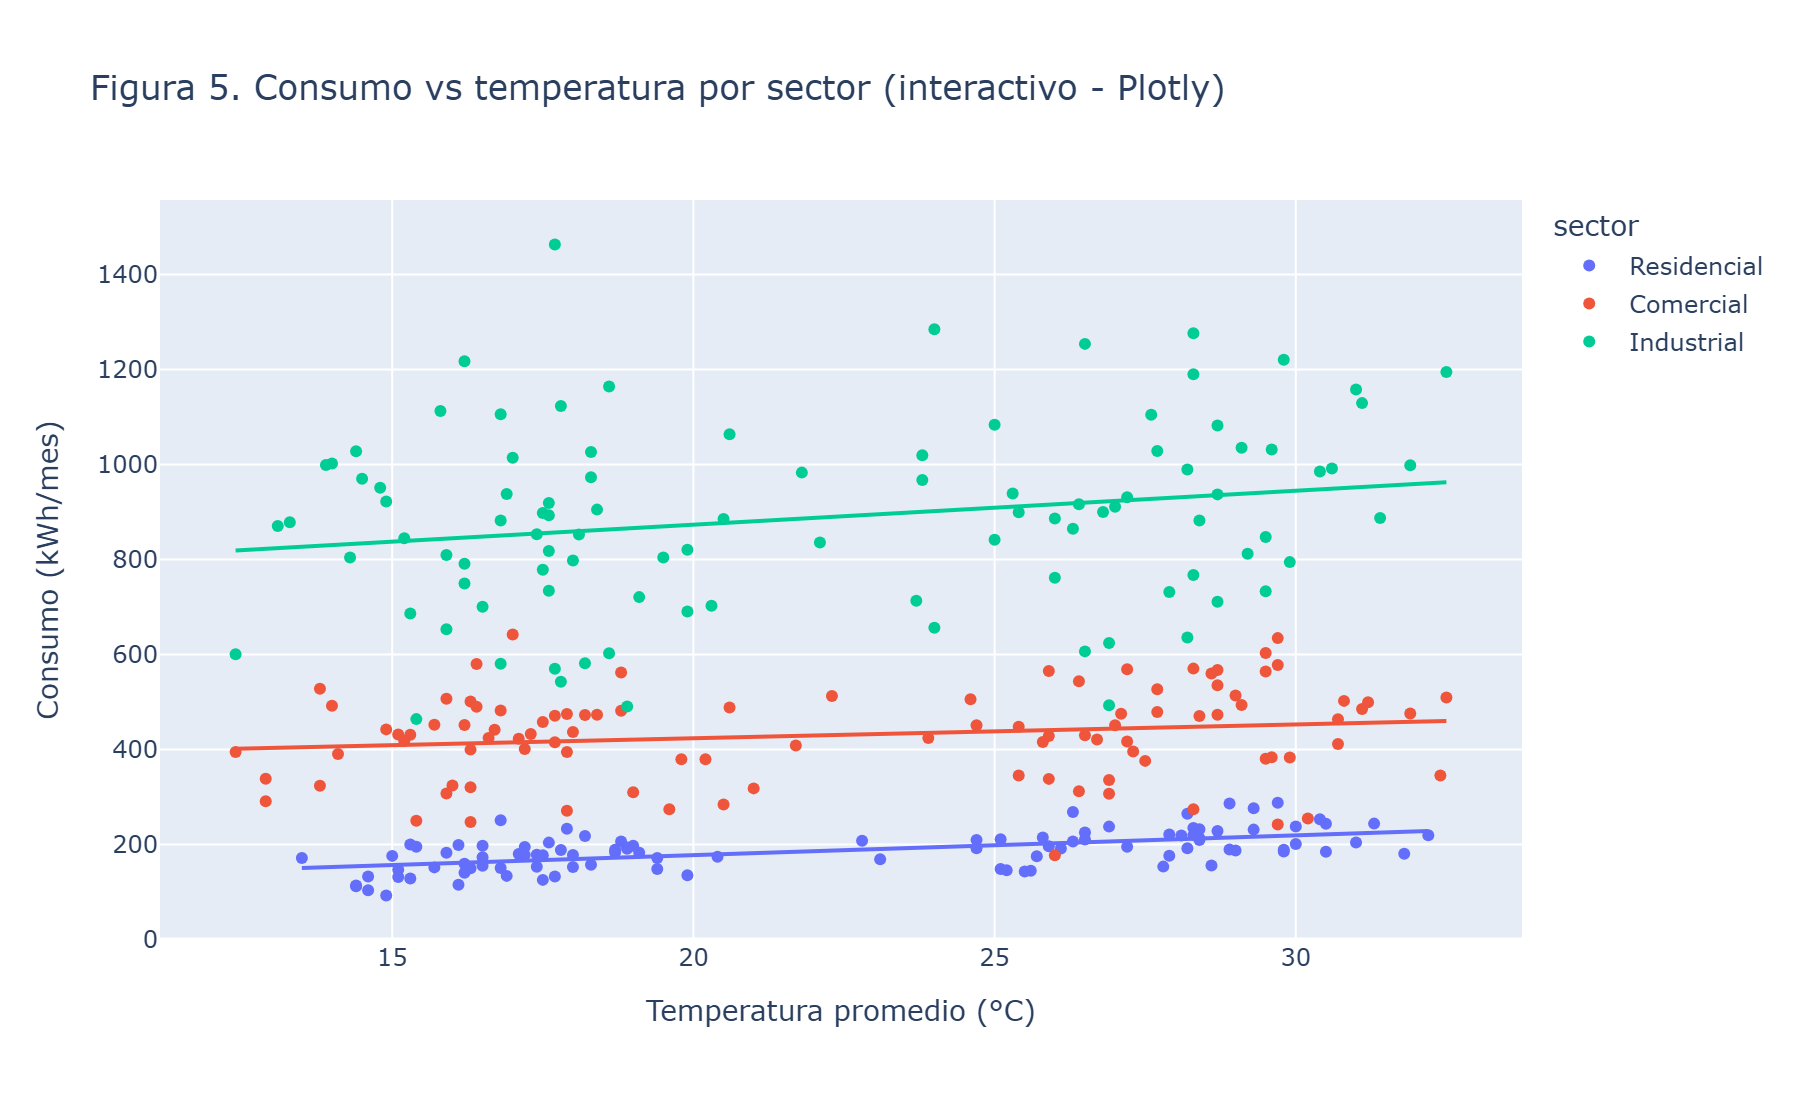
\includegraphics[width=0.82\linewidth]{assets/images/figures/python/fig5_interactivo_plotly.png}
            \caption{Consumo frente a temperatura desagregado por sector, con una
            recta de regresión ajustada dentro de cada grupo. Versión estática de la
            figura interactiva construida con Plotly, que en el navegador permite
            aislar sectores desde la leyenda, hacer zoom y consultar el
            identificador y la región de cada cliente}
            \label{fig_plotly}
        \end{figure*}

        La interactividad no es aquí un recurso decorativo. Aislar un sector desde
        la leyenda equivale a ejecutar visualmente el análisis condicionado de la
        Tabla \ref{correlacion}, y el \textit{hover} permite verificar si un punto
        extremo corresponde a una región cálida o a un cliente atípico, distinción
        que un gráfico estático obliga a resolver volviendo a los datos.

    \subsection{Por qué la correlación cae y la pendiente no}
        La explicación admite una formulación exacta. El coeficiente de Pearson y la
        pendiente de la regresión se relacionan mediante la ecuación
        (\ref{relacion_r_b}).

        \begin{equation}
            r = b_1 \, \frac{s_T}{s_Y}
            \label{relacion_r_b}
        \end{equation}

        La temperatura se asigna con independencia del sector, lo que se verifica
        contrastando su igualdad de medias entre grupos ($F = 0{,}23$; $p = 0{,}798$).
        En consecuencia, al mezclar los sectores el numerador de la ecuación
        (\ref{relacion_r_b}) apenas se altera: la pendiente global estimada es
        $b_1 = 3{,}42$, muy próxima al valor 4 fijado en la ecuación
        (\ref{generador}). Lo que cambia drásticamente es el denominador, porque la
        distancia entre los centros de los tres sectores infla la desviación
        estándar del consumo, tal como recoge la Tabla \ref{atenuacion}.

        \begin{table}[H]
            \centering
            \caption{Efecto de la agregación sobre la correlación}
            \begin{center}
                \begin{tabular}{|l|c|c|c|}
                    \hline
                    \textbf{Ámbito} & \textbf{$b_1$} & \textbf{$s_Y$} &
                    \textbf{$r$} \\
                    \hline
                    Residencial & 4,17 & 40,57  & 0,595 \\
                    \hline
                    Comercial   & 2,90 & 95,54  & 0,183 \\
                    \hline
                    Industrial  & 7,17 & 195,26 & 0,212 \\
                    \hline
                    \textbf{Global} & \textbf{3,42} & \textbf{317,49} &
                    \textbf{0,063} \\
                    \hline
                \end{tabular}
                \label{atenuacion}
            \end{center}
        \end{table}

        El mecanismo queda así identificado con precisión: \textbf{el estimador del
        efecto sobrevive a la agregación, la medida de asociación estandarizada no}.
        Con $s_T = 5{,}84$, la ecuación (\ref{relacion_r_b}) devuelve
        $3{,}42 \times 5{,}84 / 317{,}49 = 0{,}063$, exactamente el valor observado.
        No se trata, por tanto, de una inversión del signo como en la paradoja de
        Simpson clásica \cite{simpson1951interpretation}, sino de una atenuación por
        dilución: la varianza entre sectores actúa como ruido frente a una señal que
        permanece intacta \cite{kievit2013simpson}.

        \vspace{10pt}

        Conviene subrayar la asimetría práctica de este resultado. Si el objetivo
        fuera estimar cuánto aumenta el consumo por cada grado adicional, el modelo
        agregado daría una respuesta aceptable. Si el objetivo es decidir si vale la
        pena incorporar la temperatura como variable de planeación, el mismo modelo
        conduciría a descartarla. La prueba de hipótesis responde a la segunda
        pregunta y, sin la figura, lo haría de forma equivocada.

    \subsection{Verificación cruzada y reproducibilidad}
        La Tabla \ref{verificacion} compara las cifras obtenidas en ambos entornos.
        La coincidencia dígito a dígito confirma que los resultados son propiedad de
        los datos y no del software empleado.

        \begin{table}[H]
            \centering
            \caption{Verificación cruzada entre Python y R}
            \begin{center}
                \begin{tabular}{|l|l|l|}
                    \hline
                    \textbf{Prueba} & \textbf{Python} & \textbf{R} \\
                    \hline
                    Shapiro-Wilk (Res.) & 0,9912 & 0,9912 \\
                    \hline
                    t de Welch & $-23{,}5384$ & $-23{,}5384$ \\
                    \hline
                    ANOVA & $F = 775{,}9887$ & $F = 775{,}9887$ \\
                    \hline
                    Tukey (Res.$-$Ind.) & $-700{,}698$ & $-700{,}698$ \\
                    \hline
                    Pearson global & $r = 0{,}063$ & $r = 0{,}063$ \\
                    \hline
                    Varianzas & Levene $= 60{,}43$ & Bartlett $= 199{,}39$ \\
                    \hline
                \end{tabular}
                \label{verificacion}
            \end{center}
        \end{table}

        La única discrepancia corresponde a la homogeneidad de varianzas y es
        esperada, puesto que Levene se apoya en las desviaciones absolutas respecto
        de la media y Bartlett en el cociente de verosimilitudes bajo el supuesto de
        normalidad; son estadísticos distintos que en este caso conducen a la misma
        decisión. Las cinco figuras se replicaron además con ggplot2 sobre los
        estadísticos recalculados en R; la Figura \ref{fig_ggplot} presenta dos de
        ellas, que reproducen la separación entre sectores y el conjunto de
        pendientes paralelas obtenidos en Python.

        \begin{figure}[!htbp]
            \centering
            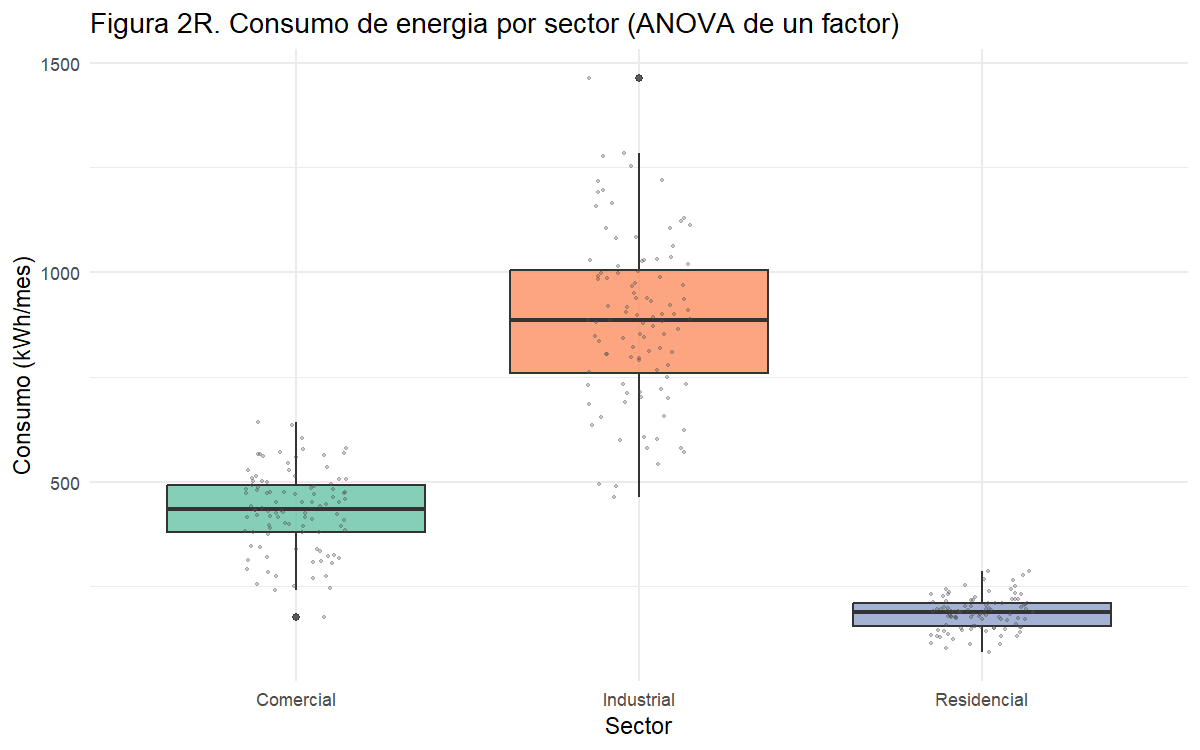
\includegraphics[width=1\linewidth]{assets/images/figures/r/fig2_boxplot_sectores.png}

            \vspace{4pt}

            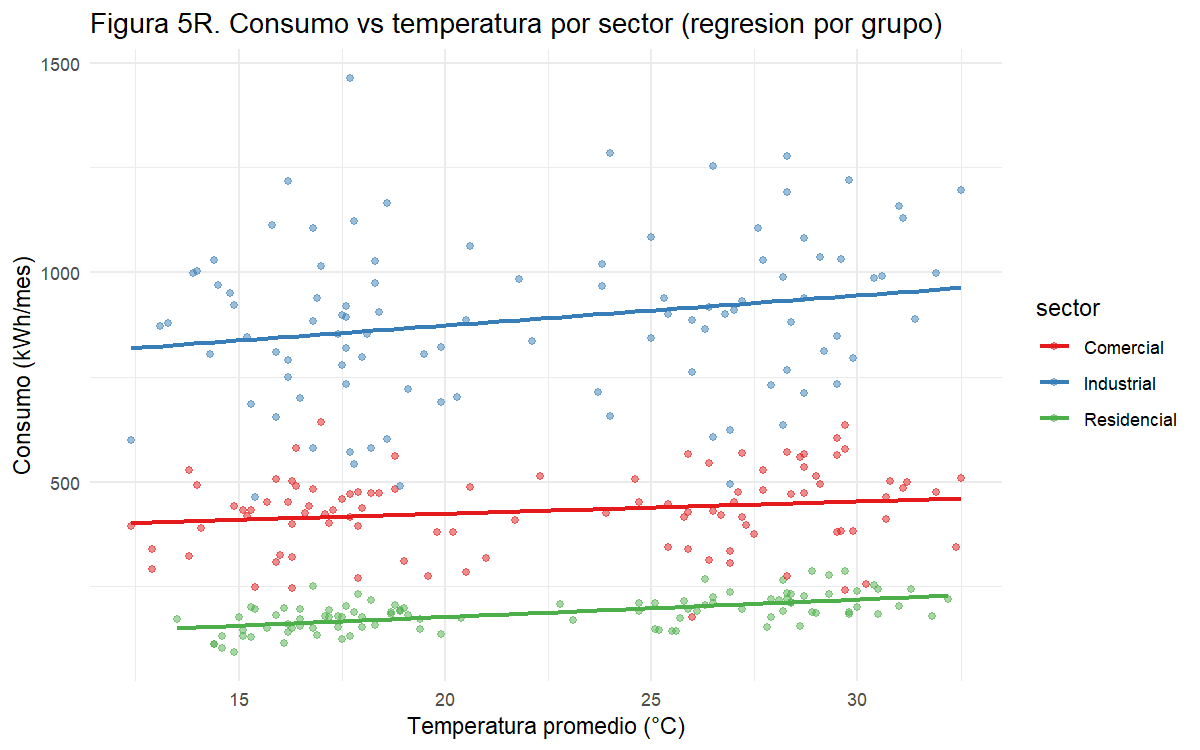
\includegraphics[width=1\linewidth]{assets/images/figures/r/fig5_dispersion_sectores.png}
            \caption{Réplicas en ggplot2 sobre los estadísticos recalculados en R:
            distribución del consumo por sector (arriba) y relación
            temperatura-consumo desagregada (abajo)}
            \label{fig_ggplot}
        \end{figure}

    \subsection{Limitaciones}
        Tres advertencias delimitan el alcance de los resultados. La primera es que
        el ANOVA clásico asume homocedasticidad, supuesto que la Tabla
        \ref{supuestos} rechaza; el diseño balanceado con $n = 100$ por grupo y la
        magnitud del estadístico ($F = 775{,}99$) hacen que la conclusión sea
        robusta, pero un contraste estricto debería recurrir al ANOVA de Welch o
        sustituir Tukey por Games-Howell \cite{montgomery2020design}. La segunda es
        que la significancia de las tres comparaciones de Tukey se ve favorecida por
        el tamaño muestral, de modo que la magnitud de las diferencias, y no su
        valor $p$, es lo que sustenta las recomendaciones. La tercera es que los
        datos son simulados y su estructura sectorial se conoce de antemano; en un
        conjunto real la variable que induce la agregación podría no estar registrada,
        lo que refuerza el argumento central de este informe, ya que la figura sería
        entonces el único indicio disponible de que el modelo agregado es inadecuado.
